\chapter{Experimental Setup}
\section{Synchrotron Radiation}
The radiation emitted by a relativistic charged particle, usually electrons, accelerated to a circular orbit through an external magnetic field is called synchrotron radiation. This radiation is polarized and emitted tangentially to the circular movement of the charged particle in forward direction. In the history of synchrotron radiation, sources have evolved from parasitic use of particle accelerators to the extend of building electron storage rings dedicated for the sole purpose of generating this radiation \cite{munro_chapter_1987}. Its most promitent features are the high brilliance, that is the number of photons per second per unit particle beam cross section and per unit solid angle within $0.1\%$ bandwidth at a specific wavelength, and its huge spectral range of emission. Depending on the energy of the relativistic particles forced on a circular orbit, in modern electron storage rings typically in the order of one to several GeV, the emission covers the range from the terahertz into the hard X-ray regime. The \gls{ptb} operates two laboratories at the dedicated sources BESSY II and the \gls{mls} \cite{brandt_metrology_2007}. The two thrid-generation synchrotron radiation sources provide maximum electron energies of $1.7$ GeV (\gls{bessy}) and $0.6$ GeV (\gls{mls}), respectively. Theoretical emission spectra for a single dipole magnet (\emph{bending magnet}) are shown in Fig.~\ref{ch_exp:fig_experimental_synchrotron_spectra} in comparison to black body radiation.
\begin{figure}
 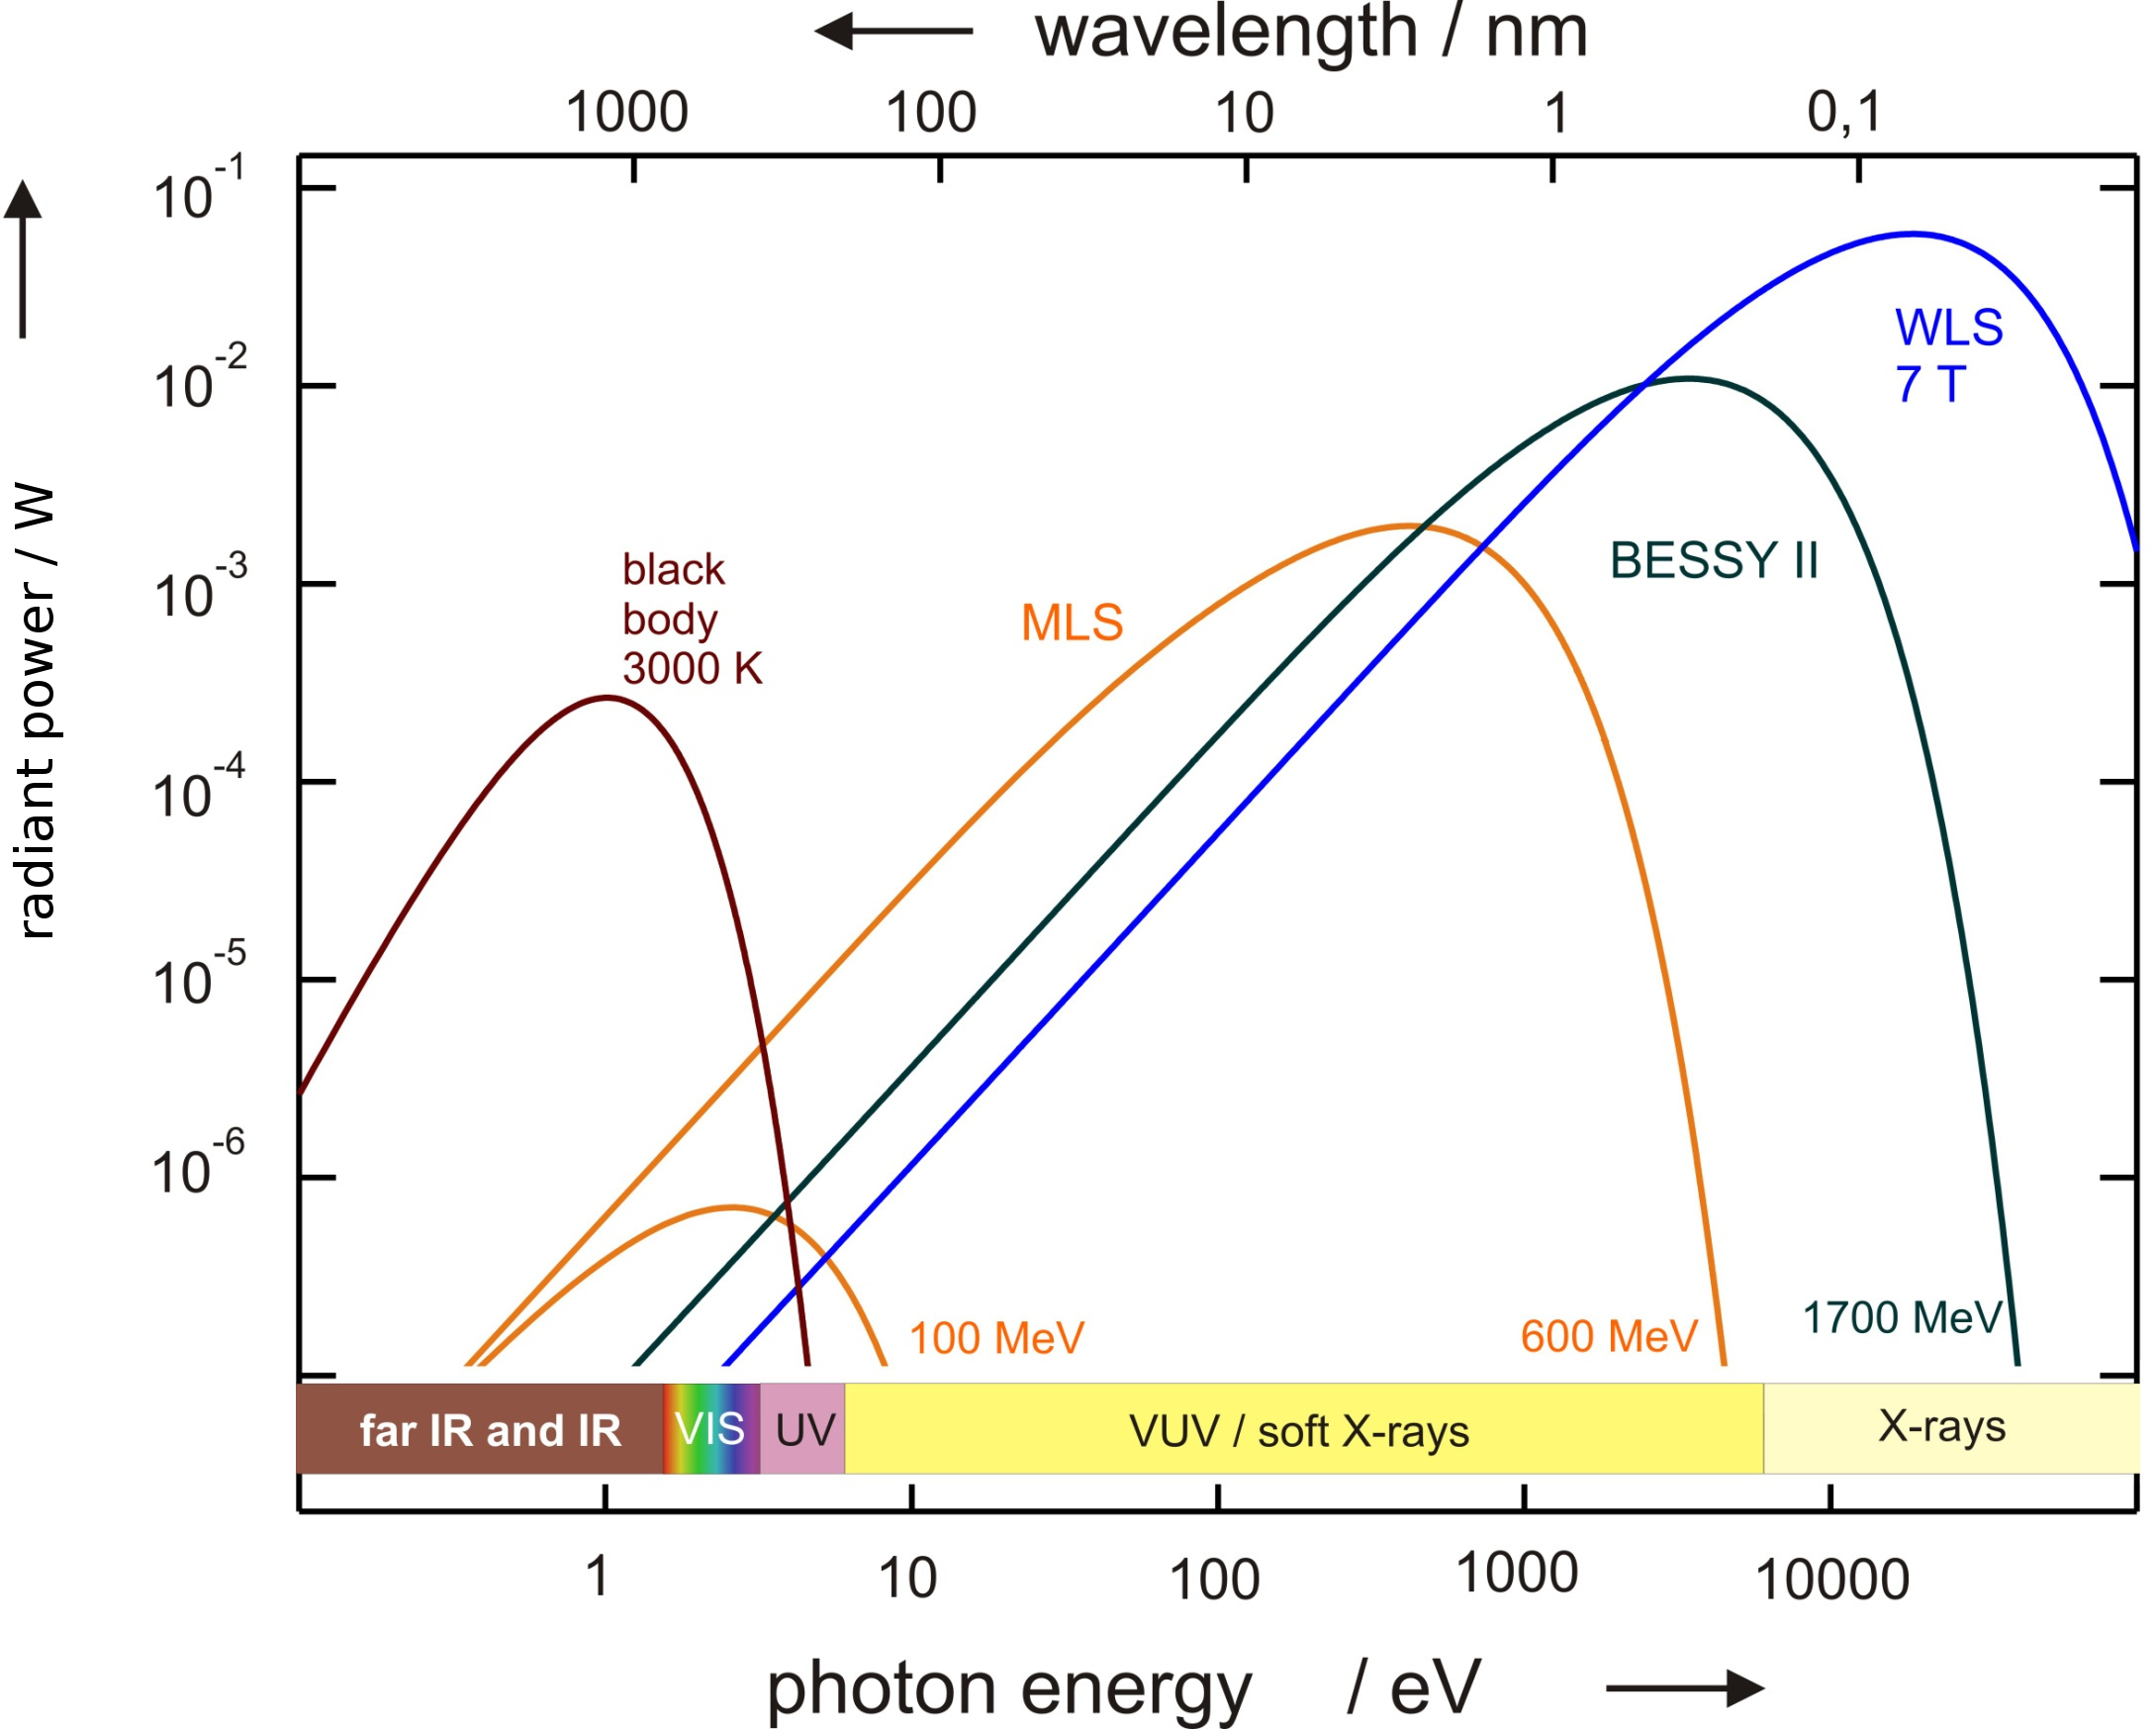
\includegraphics[width=0.7\textwidth]{img/exp-bessy-dipole-spectrum.jpeg}
 \caption[Theoretical synchrotron radiation radiant power spectra]{Theoretical synchrotron radiation radiant power spectra for the \gls{mls} and \gls{bessy} in comparison to black body radiation\footnote{Image taken from \textcite{beckhoff_quarter-century_2009}}. The curves show the radiant power of emission for bending magnets at both electron storage ring facilities for different electron energies. The curve marked WLS shows the radiant power from the $7$ Tesla wavelength shifter insertion device installed at \gls{bessy}.}
 \label{ch_exp:fig_experimental_synchrotron_spectra}
\end{figure}

A very important theoretical aspect of synchrotron radiation, apart from the high brilliance and large spectrum, is the fact that the emission can be calculated exactly from first principles of classical electrodynamics and special relativity. The theory for synchrotron radiation was developed by Schwinger \cite{schwinger_classical_1949} and we shall review its most imporant aspects here. Given all the fundamental and experimental parameters are known, the total emitted radiant power per relativistic particle can be calculated exactly as
\begin{align}
 P = \frac{1}{4 \pi \gls{epsilon_0}} \frac{2}{3} \frac{\gls{e}^2 \gls{c}}{R^2}\Big( \frac{E}{\gls{m_0} \gls{c}^2}\Big)^4 \text{,} \label{ch_exp:schwinger_equation_total_power}
\end{align}
where \gls{e} is the elementary charge, \gls{c} is the speed of light in vacuum, $E$ is the particles energy, \gls{m_0} is the rest mass of the particle and $R$ is the radius of the circular trajectory imposed by the magnetic field. The radiant power is thus inversely proportional to the fourth power of the particles rest mass, which explains the usage of light electrons in comparison with significanlty heavier protons in synchrotron radiation sources. The dependence on the electron energy is visible in another characteristic value for the emitted radiant power, visible as a shift to higher photon energies (smaller wavelengths) in Fig.~\ref{ch_exp:fig_experimental_synchrotron_spectra}, known as the critical energy or critical wavelength \cite{schwinger_classical_1949}, respectively,
\begin{align}
 E_C = \frac{3 \gls{h} \gls{c}}{4 \pi R} \Big( \frac{E}{\gls{m_0} \gls{c}^2}\Big)^3 \text{.} \label{ch_exp:characteristic_energy}
\end{align}
It marks the point in the spectrum, where the integrated radiant power for all values above and below the critical energy are equal \cite{balerna_introduction_2015}. This formula quantifies the shift towards higher energies due to the increase of the electron energy comparing the \gls{mls} and \gls{bessy} emission spectra. Apart from the spectral distribution, the emitted radiation is linearly polarized with an electric field vector oscillating parallel to the plane of the circular orbit. This property, however, is only stricly valid for the emission inside this plane. For radiation above or below, a vertical polarization component (parallel to the surface normal of the orbital plane) exsists. The energy $W$ emitted by a single electron on a circular orbit per unit solid angle $\text{d} \Omega$ and per unit angular frequency interval $\text{d} \omega$ is described by
\begin{align}
 \frac{\text{d}^2 W}{\text{d} \Omega \text{d} \omega} &= \frac{\gls{e}^2 R^2}{36 \pi^3 \gls{epsilon_0} \gamma^4} \omega^2 \big(1+ (\gamma \Psi)^2\big)\Big( K_{2/3}^2(\zeta) + \frac{(\gamma \Psi)^2}{1 + (\gamma \Psi)^2} K_{1/3}^2(\zeta)\Big) \text{,} \label{ch_exp:schwinger_equation_spectral}
\end{align}
where $\gamma = \sfrac{E}{\gls{m_0} \gls{c}^2}$ and $\Psi$ is the angle between the orbital plane and the observation direction outside of that plane \cite{schwinger_classical_1949}. The argument of the modified Bessel funktions of second kind $K_{x}(\zeta)$ is defined as
\begin{align}
 \zeta = \frac{R \omega}{3 c \gamma^3} \big(1 + (\gamma \Psi)^2\big)^\frac{3}{2} \text{.}
\end{align}


The ability to calculate the exact emission and polarization properties of synchrotron radiation based on Eq.~\eqref{ch_exp:schwinger_equation_spectral} with a given electron current and aceptance angle have another very valuable side effect for the field of metrology. It enables the use of synchrotron radiation as a primary standard for electromagnetic radiation within the available spectral range, which is in fact exploited by the \gls{ptb} \cite{thornagel_electron_2001} to provide absolute radiometry.

The dedicated sychrotron radiation facilities, such as \gls{bessy} and the \gls{mls} provide additional possibilities of generating synchrotron radiation beyond a simple bending magnet through different instertion devices. Fig.~\ref{ch_exp:fig_bessy2} gives a shematic overview over the storage ring \gls{bessy}. At each of the marked dipole magnets, synchrotron radiation is produced according the theory presented above. The radiation is transmitted through outlet systems towards a large number of beamlines, which monochromatize and focus the radiation for experimental applications.
\begin{figure*}[htb]
    \def\svgwidth{0.7\textwidth}
    \import{svg/}{bessy.pdf_tex}
    \caption[Schematic overview of BESSY II.]{Schematic overview of the electron storage ring facility \gls{bessy}\footnote{Original image by \gls{hzb}, Ela Strickert, source: \url{https://www.helmholtz-berlin.de/mediathek/bildarchiv/}}. The synchrotron accelerates the electrons coming from the \gls{linac}, which are then injected in the electron storage ring with their full desired energy. Electromagnetic lenses focus and stabilize the beam, as well as deflecting it onto the circular orbit while emitting synchrotron radiation at each dipole (bending) magnet. Cavities reaccelerate the electrons in the storage ring to compensate the energy loss due to the radiation emission.}
    \label{ch_exp:fig_bessy2}
\end{figure*}
Undulators or wigglers are inserted in the straight sections of the \gls{bessy} storage ring with a large number of periodically arranged magnets with alternating polarization forcing the electrons on a sinosoidal beam path. The goal of these insertion devices is to shift the critical energy of the storage ring towards higher energies (wigglers) or to dramatically increase the brilliance within a significantly smaller spectral range compared to bending magnets (undulators). The different effect of the undulators and wigglers on the generated spectrum is determined by the magnetic field strength $B_0$ and the distance between two identical periodic arragnements of the magnets of alternating polarization $\lambda_0$. The deflection parameter quantifies this relation through $K \propto B_0 \lambda_0$. Undulators typically have deflection parameters $K < 1$ while in case of wigglers $K \gg 1$ \cite{munro_chapter_1987}. Technically, the magnetic field strength can be varied by changing the distance (``gap'') between the magnets vertically. By changing the vertical alignment of the magnetic field direction with respect to the beam path, it is even possible to affect the polarization properties of the emitted radiation to obtain circularly or eliptically polarized radiation.
\begin{figure}[htb]
    \def\svgwidth{0.7\textwidth}
    \import{svg/}{mls.pdf_tex}
    \caption[Schematic overview of the MLS]{Schematic overview of the electron storage ring facility \gls{mls}}
    \label{ch_exp:fig_mls}
\end{figure}


The most advanced light source available today, also known as fourth generation source, is following the concept of a \gls{fel} as first invented by \textcite{madey_stimulated_1971}. In that case radiation is produced by a typically single very long undulator inside a linear accelerator instead of a comparatively short straight section of a storage ring. The concept was first demonstrated by \textcite{deacon_first_1977}. \Gls{fel} sources produce highly coherent radiation in the x-ray regime through the principle of \gls{sase} \cite{derbenev_possibility_1982, bonifacio_collective_1984}. Here, the emitted radiation inside the long undulator has a feedback effect on the electron bunch travelling along the beam path. The result is a microbunching of the electron cloud through the electric field of the emitted radiation connected with a (random) wavelength within a certain spectral range defined by the undulator properties. The microbunching causes amplification of that wavelength, which causes an emission spectrum showing several spikes of amplified wavelengths with a noisy background until a saturation level is reached \cite{milton_exponential_2001}.


\section{The SX700 and EUVR Beamlines}
The radiation generated in bending magnets or in insertion devices in synchrotron radiation sources typically requires monochromatization and focussing trough a series of optical elements depending on the experimental requirements or designated use cases. The two \gls{ptb} beamlines for the \gls{euv} spectral range at the two storage rings \gls{bessy} and \gls{mls} operate on the broad spectrum emitted by bending magnets at each facility. The \gls{sx700} at \gls{bessy} provides a monochromatic beam in the spectral range from $\nm{0.7}$ to $\nm{41.3}$ wavelength (corresponding to photon energy range from $\ev{30}$ to $\ev{1800}$) \cite{beckhoff_quarter-century_2009}. The total radiation power and the corresponding relative bandwidth at that beamline are shown in Fig.~\ref{ch_exp:fig_flux_sx700}. The beam size at the entrance aperture to the reflectometer (experimantal end station) is variable through the setting of the exit slits. In the standard setting is approximately \mm{1} by \mm{1} \cite{scholze_high-accuracy_2001} and can be reduced to \mm{0.1} vertical extent (grating dispersion direction) and \mm{0.5} horizontal extent.
\begin{figure}[htb]
    \def\svgwidth{0.7\textwidth}
    \import{svg/}{flux_sx700.pdf_tex}
    \caption[Radiant power and relative bandwidth of the SX700 beamline.]{Radiant power and relative bandwidth of the SX700 beamline at \gls{bessy} \footnote{Original image taken from \textcite{scholze_high-accuracy_2001}}.}
    \label{ch_exp:fig_flux_sx700}
\end{figure}

The monochromatization of the radiation is achieved by a plane grating monochromator with a blazed line grating with 1200 lines per millimeter mounted with its rotational axis within the plane of the storage ring and illuminated perpendicular to the grating lines determining the dispersive direction. The schematic layout of the beamline is illustrated in Fig.~\ref{ch_exp:fig_sx700_schematic} including the plane grating position of the monochromator. For the purpose of suppression of higher grating orders, additional filters are installed close to the entrance aperture to the experimental station.
\begin{figure*}[htb]
    \def\svgwidth{\textwidth}
    \import{svg/}{sx700_scheme.pdf_tex}
    \caption[Schematic setup of the SX700 beamline.]{Schematic setup of the \gls{sx700} beamline at \gls{bessy} in top view (upper part) and side view (lower part) \footnote{Original image taken from \textcite{scholze_high-accuracy_2001}}.}
    \label{ch_exp:fig_sx700_schematic}
\end{figure*}

\section{The ELLI and BigRef Reflectometers}
\begin{figure*}[htb]
    \def\svgwidth{\textwidth}
    \import{svg/}{elli.pdf_tex}
    \caption[The EUV ellipso-scatterometer.]{The EUV ellipso-scatterometer.}
    \label{ch_exp:fig_elli}
\end{figure*}
BigRef \cite{scholze_high-accuracy_2001}
ELLI \cite{soltwisch_polarization_2015}
\section{Grazing-incidence X-ray Fluorescence at the FCM Beamline}

\section{Sample systems}
\begin{figure}[htb]
        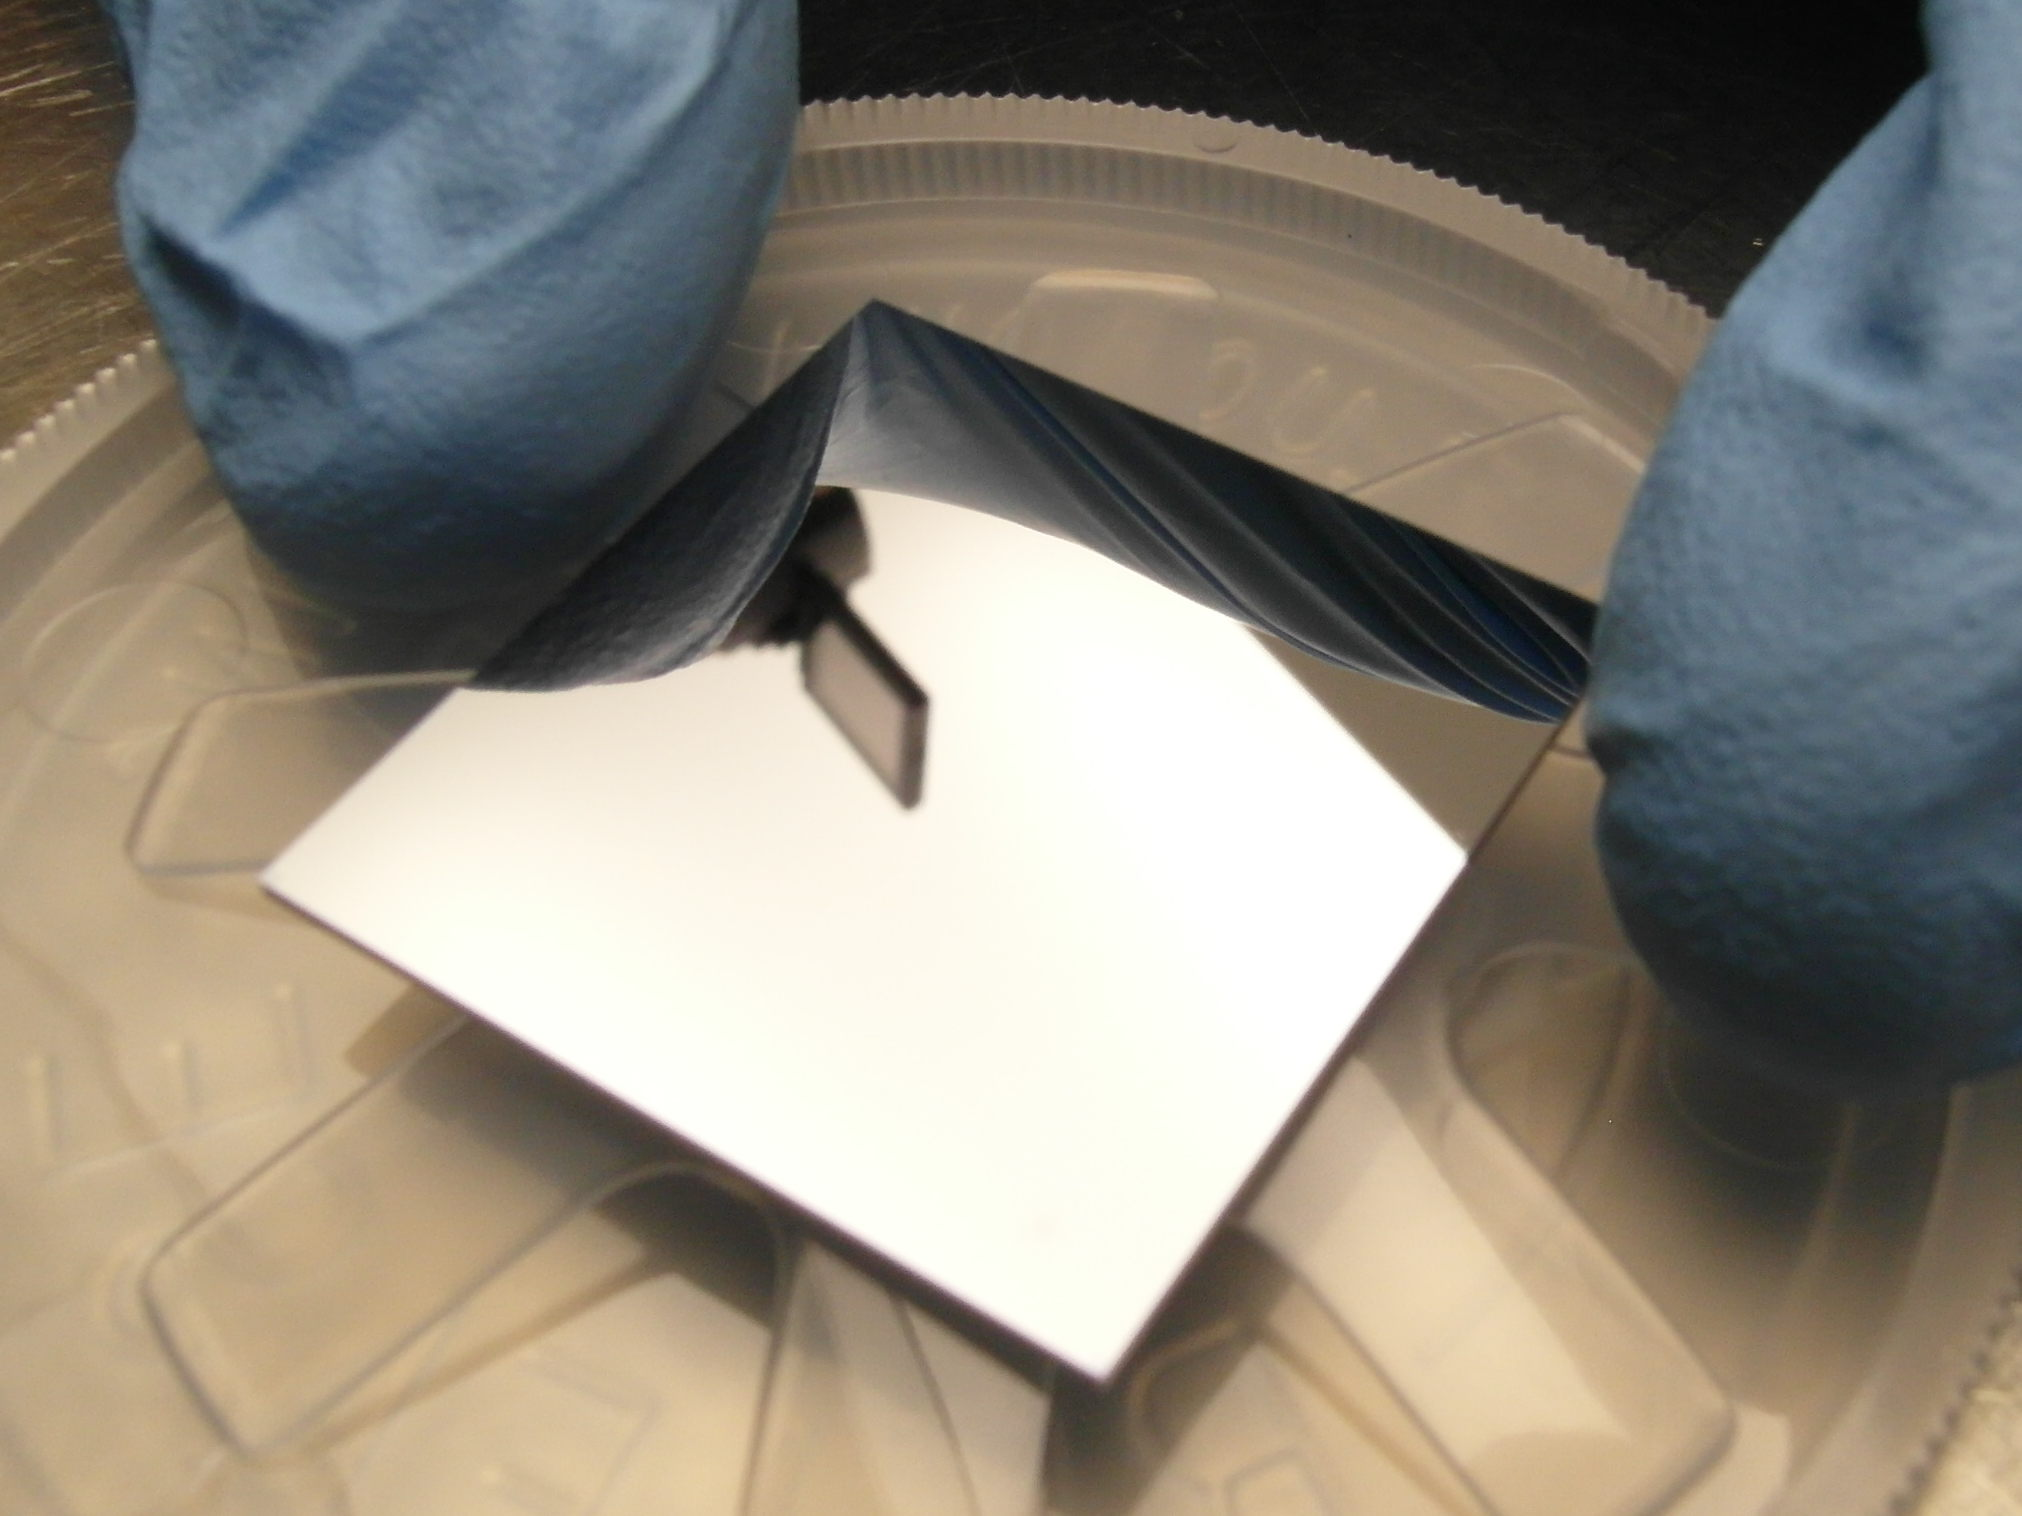
\includegraphics[width=0.4\textwidth]{img/SAM_1910_v1}
        \caption[Mo/Si multilayer sample.]{%
            Mo/Si multilayer sample.}
        \label{ch_exp:fig_mosi_sample}
\end{figure}
\begin{enumerate}
 \item Mo/Si mirrors for $13.5$ nm for EUV lithography and other applications
 \item Cr/Sc for the water window, protein contrast in water, mirrors with bad performance, curved, etc.
\end{enumerate}
